\documentclass[11pt,letter]{article}
\usepackage[utf8]{inputenc}
\usepackage{amsmath}
\usepackage{amsfonts}
\usepackage{amssymb}
\usepackage{enumerate}
\usepackage{graphicx}


\usepackage[pages=all]{background}
% configuración
\backgroundsetup{
 scale=1, %escala de la imagen, es recomendable que sea del mismo tamaño que el pdf
 color=black, %fondo a usar para transparencia
 opacity=1.0, %nivel de transparencia
 angle=0, %en caso de querer una rotación
 contents={%
  \includegraphics[width=\paperwidth,height=\paperheight]{fondo} %nombre de la imagen a utilizar como fondo
 }%
}



\begin{document}
\title{Proyecto4}
\begin{center}
\textbf{\LARGE Universidad Aut\'onoma del Estado de M\'exico}\\[1cm] 
\large \textbf{Centro Universitario UAEM Zumpango}\\[1cm]
\large \textbf{Ingenier\'ia en Computaci\'on}\\[1cm]
\large \textbf{Fisica Basica}\\[0.5cm] 
\large \textbf{Magaña Alcudia Ana Aurora}\\
\large \textbf{Valenzuela Ju\'arez Axel}\\[1cm]
\large \textbf{Proyecto4: Problema 4}\\[1cm]
\large \textbf{Profesor:}\\[0.5cm]
\large \textbf{Asdr\'ubal L\'opez Chau}\\[1.2cm]
\large \textbf{Fecha de entrega: 03 de Junio del 2018}



\end{center}
\newpage
\section*{Problema 4}
Una fuerza $F$ es usada para sostener un bloque de masa m sobre un plano inclinado. El plano forma un \'angulo con la horizontal y $F$ es perpendicular al plano. El coeficiente de fricción entre el plano y el bloque es $\mu$ .¿Cu\'al es la m\'inima fuerza F, necesaria para mantener el bloque en reposo?\\
\begin{enumerate}[a)]
\item $\mu mg$
\item $mg cos\Theta $
\item $mg sen\Theta $
\item $(mg/\mu)sen\Theta $
\item $(mg/\mu)(sen\Theta -\Theta) $
\end{enumerate}
\begin{figure}[h]
  \centering
  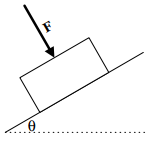
\includegraphics{imagen1}
      \caption{Representaci\'on}
\end{figure}
\subsection*{Soluci\'on:}
\begin{center}
Se obtiene las fuerzas que actuan en el eje $"y"$ para sacar la normal.
$$N = mg cos \Theta + F$$
$Fx$ debe ser igual a 0 para que este en equilibrio asi que se iguala a 0.
$$Fx = 0$$
Se sustituyen valores en $Fx $ por las fuerzas que actuan en el eje $"x"$.
$$Fs = mg sen \Theta ...(1)$$
$$Fs - mg sen\Theta = 0$$
Se iguala Fs con los valores de $(\mu)(N)$.
$$Fs = \mu_s * N$$
Se sustituye el valor de F con la ecuacion 1.
$$mg sen\Theta = \mu_s * N...(2)$$
Se despeja la normal de la ecuacion 2.
$$N = \frac{mg sen\Theta}{\mu_s}...(3)$$
Se hacen la sumatoria de fuerzas para el eje $"y"$
$$Fy = 0$$
$$-F - mg cos\Theta + N=0...(4)$$
Se despeja F de la ecuacion 4 y se sustituye el valor de N por la ecuacion 3.
$$F = \frac{mg sen\Theta}{\mu_s} - mg cos\Theta$$
Lo cual es igual a la opcion e.
$$F = \frac{mg sen\Theta}{\mu_s} - mg cos\Theta=(mg/\mu)(sen\Theta -\Theta)$$
\begin{figure}[h]
  \centering
      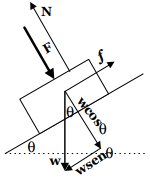
\includegraphics[scale=0.9]{imagen2}
            \caption{Representaci\'on de soluci\'on}
\end{figure}
\end{center}
\newpage
\section*{Conclusion}
Qt es muy f\'acil de usar y genera interfaces con una muy buena vista, as\'i como en particular para llegar a la soluci\'on del problema seleccionado se necesit\'o de conocimientos de leyes de newton el cual es un tema visto en clase, haciendo que resolver el problema fuera muy f\'acil, siendo lo m\'as tedioso plasmar la soluci\'on en el programa de Qt.

En conclusi\'on, tener conocimientos de f\'isica para el ingeniero en computaci\'on es algo necesario y evidentemente muy importante para la soluci\'on de diversos problemas en la vida real y en muchos problemas a realizar.

\newpage
\section*{Referencias}
qt. (2018). doc.qt.io. Obtenido de http://doc.qt.io/qtcreator/creator-editor-functions.html
\\

Enlace a GitHub: https://github.com/AntiDesert5/Problema04.git
\end{document}